\documentclass{ctexart}
\usepackage{geometry}
\usepackage{fancyhdr}
\usepackage{graphicx}
\usepackage{booktabs}
\usepackage{amsmath}
\usepackage{multirow}
\usepackage{caption}
\usepackage{tikz}
\usepackage{array}
\xeCJKsetup{CJKmath=true} 
\usepackage{zhnumber} % change section number to chinese
\renewcommand\thesection{\zhnum{section}}
\renewcommand \thesubsection {\arabic{subsection}}
\CTEXsetup[format={\Large\bfseries}]{section}

\geometry{
    a4paper,
    left=3.18cm,
    right=3.18cm,
    top=3.04cm,
    bottom=3.04cm
}

\pagestyle{fancy}
\fancyhf{}
\renewcommand{\headrulewidth}{0.7pt} % 设置页眉横线粗细
\fancyhead[L]{\kaishu\large 大学物理实验报告} % 在左侧设置页眉文字
\fancyhead[R]{\kaishu\large 哈尔滨工业大学(深圳) } % 在右侧设置页眉文字
\fancyfoot[R]{\thepage} % 将页数放在右下角


\setlength\headwidth{\textwidth}

\begin{document}

\noindent
\textbf{
    \begin{tabular}{p{2.4cm}p{2.4cm}p{4cm}p{3.8cm}}
        班级 \hrulefill & 学号 \hrulefill & 姓名 \hrulefill & 教师签字 \hrulefill \\
    \end{tabular}\\
    \begin{tabular}{p{6cm}p{3.6cm}p{3.55cm}}
        \ 实验日期 \hrulefill & 预习成绩 \hrulefill & 总成绩 \hrulefill
    \end{tabular}\\
}
\rule[-10pt]{\textwidth}{0.7pt}

\begin{center}
    \Large \textbf{实验内容 \underline{光电效应法测定普朗克常量}}
\end{center}

\section{预习内容}

\subsection{请简单推导一下本实验中光频率$\nu$与对应截止电压$U_0$的关系。}
\subsection{实验中光电流的实测值与理论值有所区别,产生原因是什么?在测量截止电压时如何消除此影响。}

\newpage
\section{实验现象及原始数据记录}

\begin{table}[!h]
    \centering
    \renewcommand{\arraystretch}{1.5} % 表格行高倍数
    \caption{截止电压测量(光阑孔直径 = 2 mm)}
    \begin{tabular}{|c|m{1.5cm}<{\centering}|m{1.5cm}<{\centering}|m{1.5cm}<{\centering}|m{1.5cm}<{\centering}|m{1.5cm}<{\centering}|}
        \hline
        光波长 $\lambda \ (mm)$ & 365.0 & 404.7 & 435.8 & 546.1 & 577.0 \\
        \hline
        光频率 $\nu \ (\times 10^{14} Hz)$ & 8.216 & 7.410 & 6.882 & 5.492 & 5.196 \\
        \hline
        截至电压 $ U_c \ (V)$ & & & & & \\
        \hline
    \end{tabular}
\end{table}

\begin{table}[!h]
    \centering
    \renewcommand{\arraystretch}{1.5} % 表格行高倍数
    \caption{截止电压测量(光阑孔直径 = 4 mm)}
    \begin{tabular}{|c|m{1.5cm}<{\centering}|m{1.5cm}<{\centering}|m{1.5cm}<{\centering}|m{1.5cm}<{\centering}|m{1.5cm}<{\centering}|}
        \hline
        光波长 $\lambda \ (mm)$ & 365.0 & 404.7 & 435.8 & 546.1 & 577.0 \\
        \hline
        光频率 $\nu \ (\times 10^{14} Hz)$ & 8.216 & 7.410 & 6.882 & 5.492 & 5.196 \\
        \hline
        截至电压 $ U_c \ (V)$ & & & & & \\
        \hline
    \end{tabular}
\end{table}

\begin{table}[!h]
    \centering
    \renewcommand{\arraystretch}{1.5} % 表格行高倍数
    \caption{截止电压测量(光阑孔直径 = 8 mm)}
    \begin{tabular}{|c|m{1.5cm}<{\centering}|m{1.5cm}<{\centering}|m{1.5cm}<{\centering}|m{1.5cm}<{\centering}|m{1.5cm}<{\centering}|}
        \hline
        光波长 $\lambda \ (mm)$ & 365.0 & 404.7 & 435.8 & 546.1 & 577.0 \\
        \hline
        光频率 $\nu \ (\times 10^{14} Hz)$ & 8.216 & 7.410 & 6.882 & 5.492 & 5.196 \\
        \hline
        截至电压 $ U_c \ (V)$ & & & & & \\
        \hline
    \end{tabular}
\end{table}

\begin{tikzpicture}[remember picture,overlay]
    \node[anchor=south east,inner sep=100pt] at (current page.south east) {
        \renewcommand{\arraystretch}{1.5} % 表格行高倍数
        \setlength{\tabcolsep}{18pt}    
    \begin{tabular}{|c|c|}
        \hline
        \LARGE  教师 & \LARGE  姓名 \\
        \hline
        \LARGE \kaishu 签字 &  \\
        \hline
        \end{tabular}
    };
\end{tikzpicture}

\newpage

\section{数据处理}

(在三个不同直径的光阑孔下分别测量对应各个光频率$\nu$的截止电压$U_0$,找出两者的线性关系。用最小二乘法与作图法求出普朗克常数$h$的实验值,以及与普朗克常数标准值$h_0 = 6.626 \times 10^{-34} J \cdot s$的相对误差。)

\begin{figure}[h!]
    \centering
    \begin{minipage}[b]{0.45\textwidth}
        \centering
        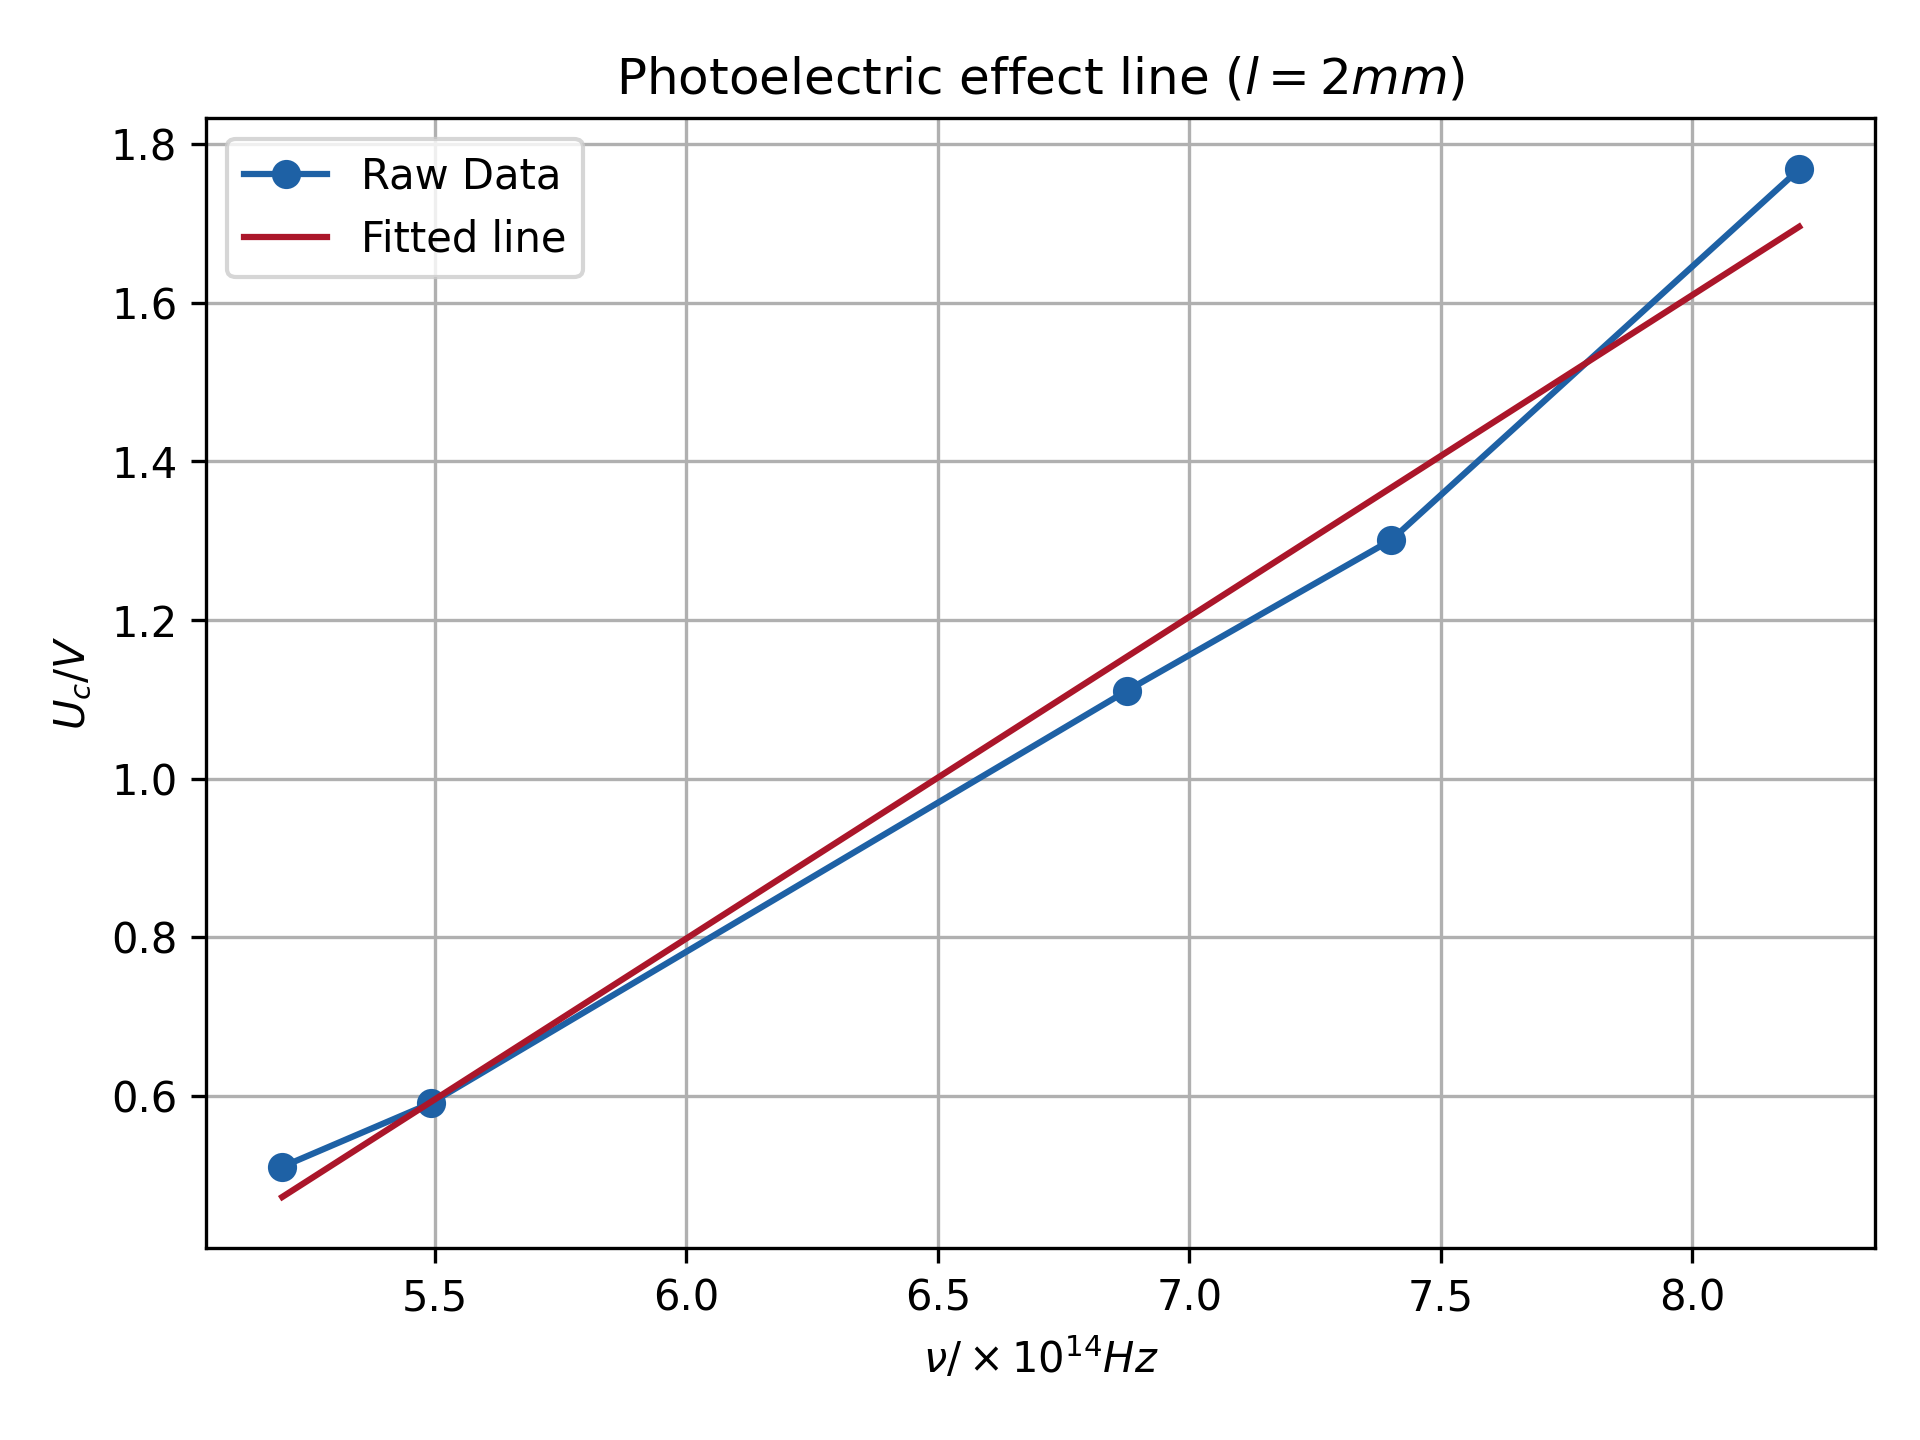
\includegraphics[width=\textwidth]{l_2.png}
        \caption{光阑孔直径 = 2 mm}
    \end{minipage}
    \hfill
    \begin{minipage}[b]{0.45\textwidth}
        \centering
        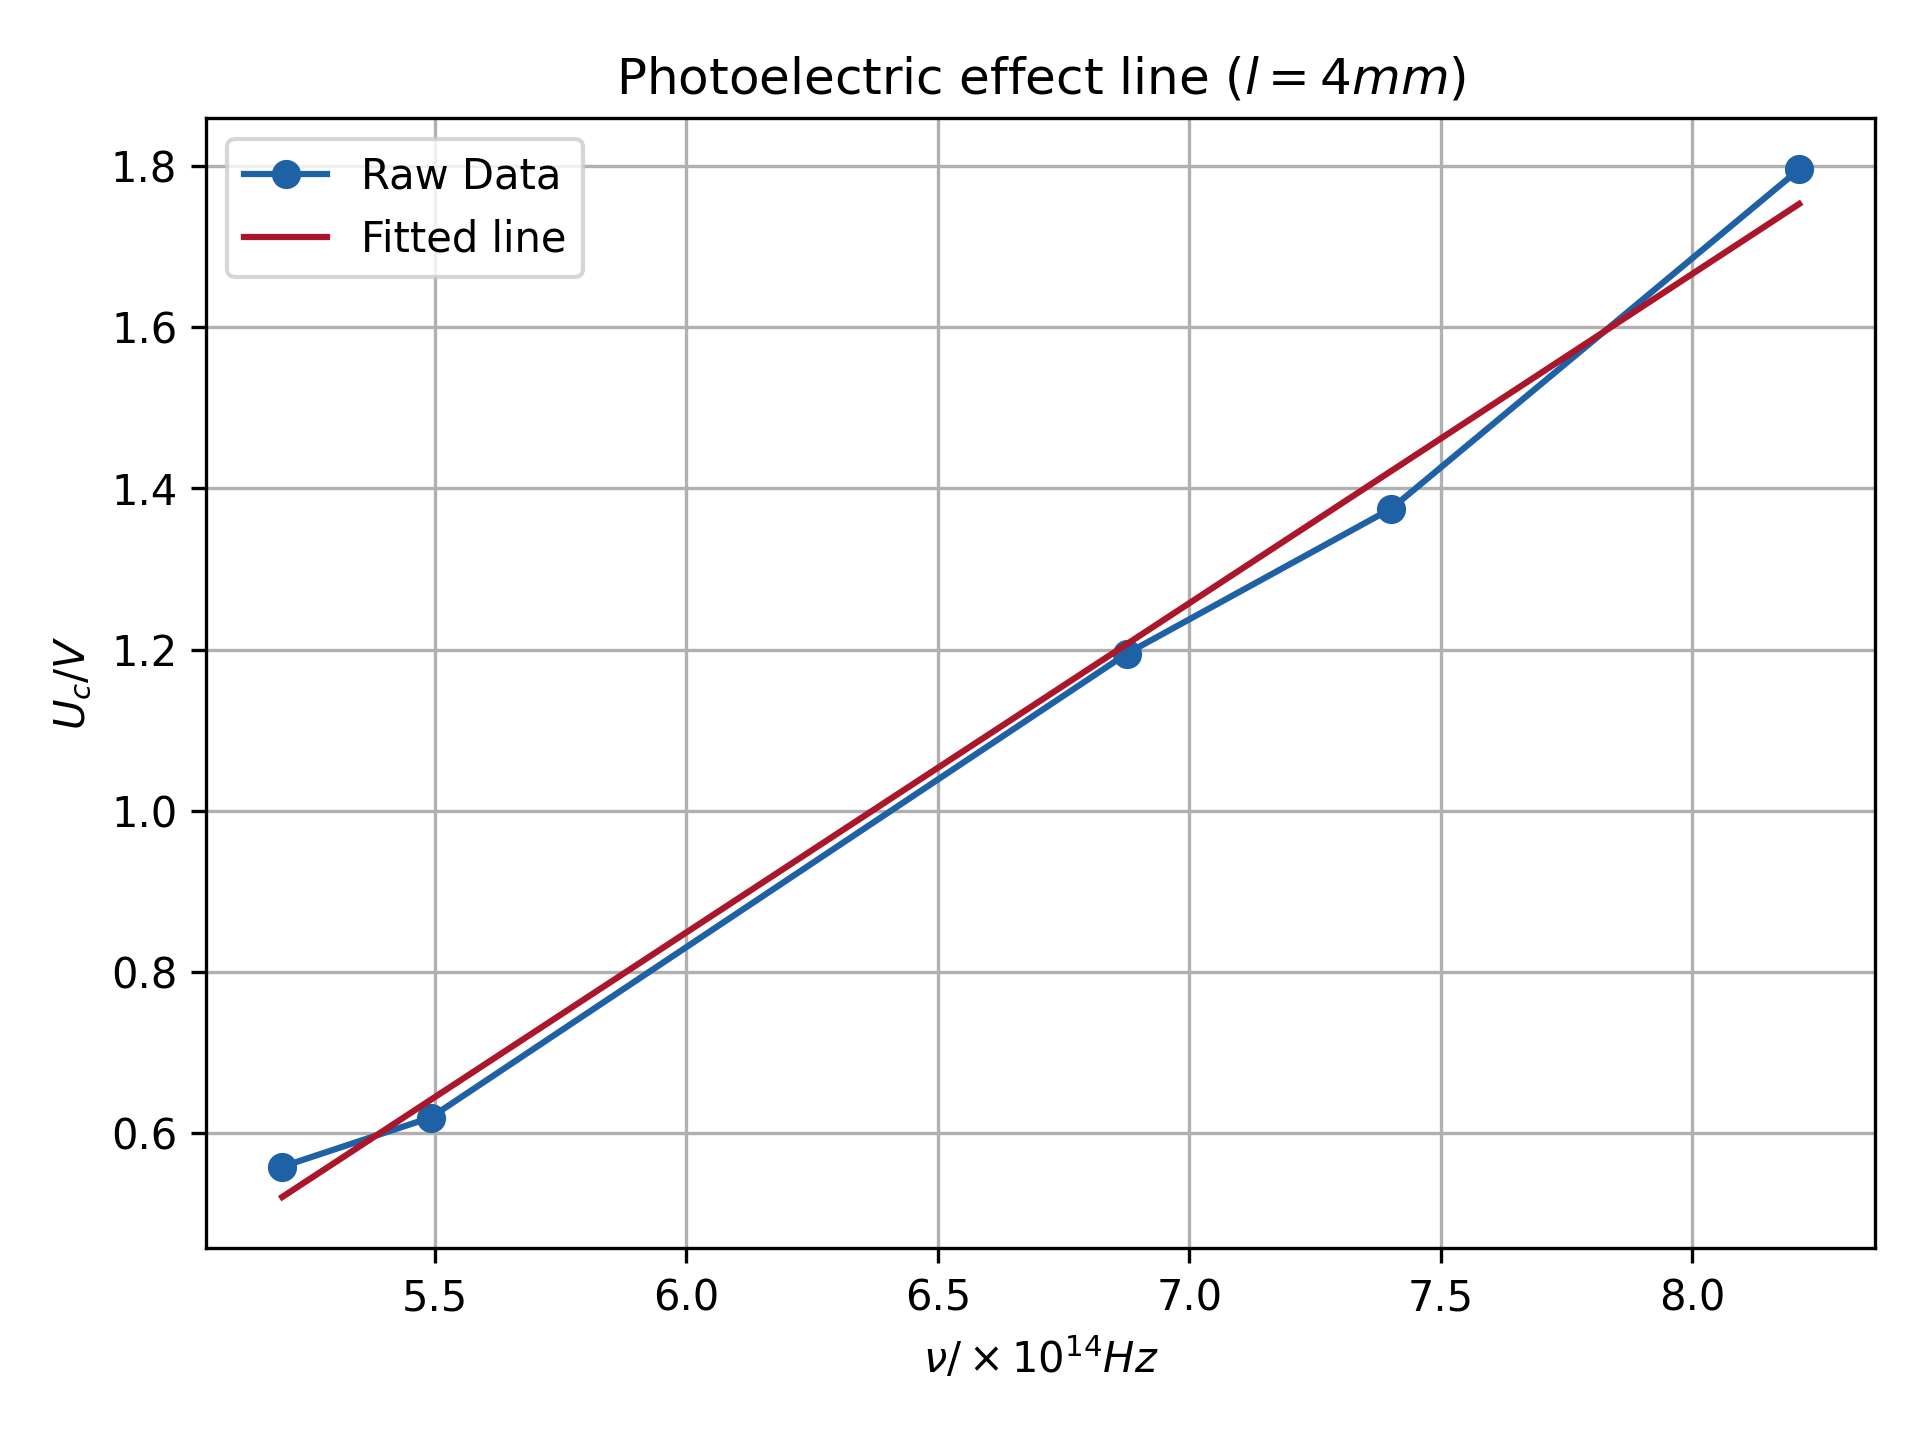
\includegraphics[width=\textwidth]{l_4.png}
        \caption{光阑孔直径 = 4 mm}
    \end{minipage}
    \vfill
    \begin{minipage}[b]{0.45\textwidth}
        \centering
        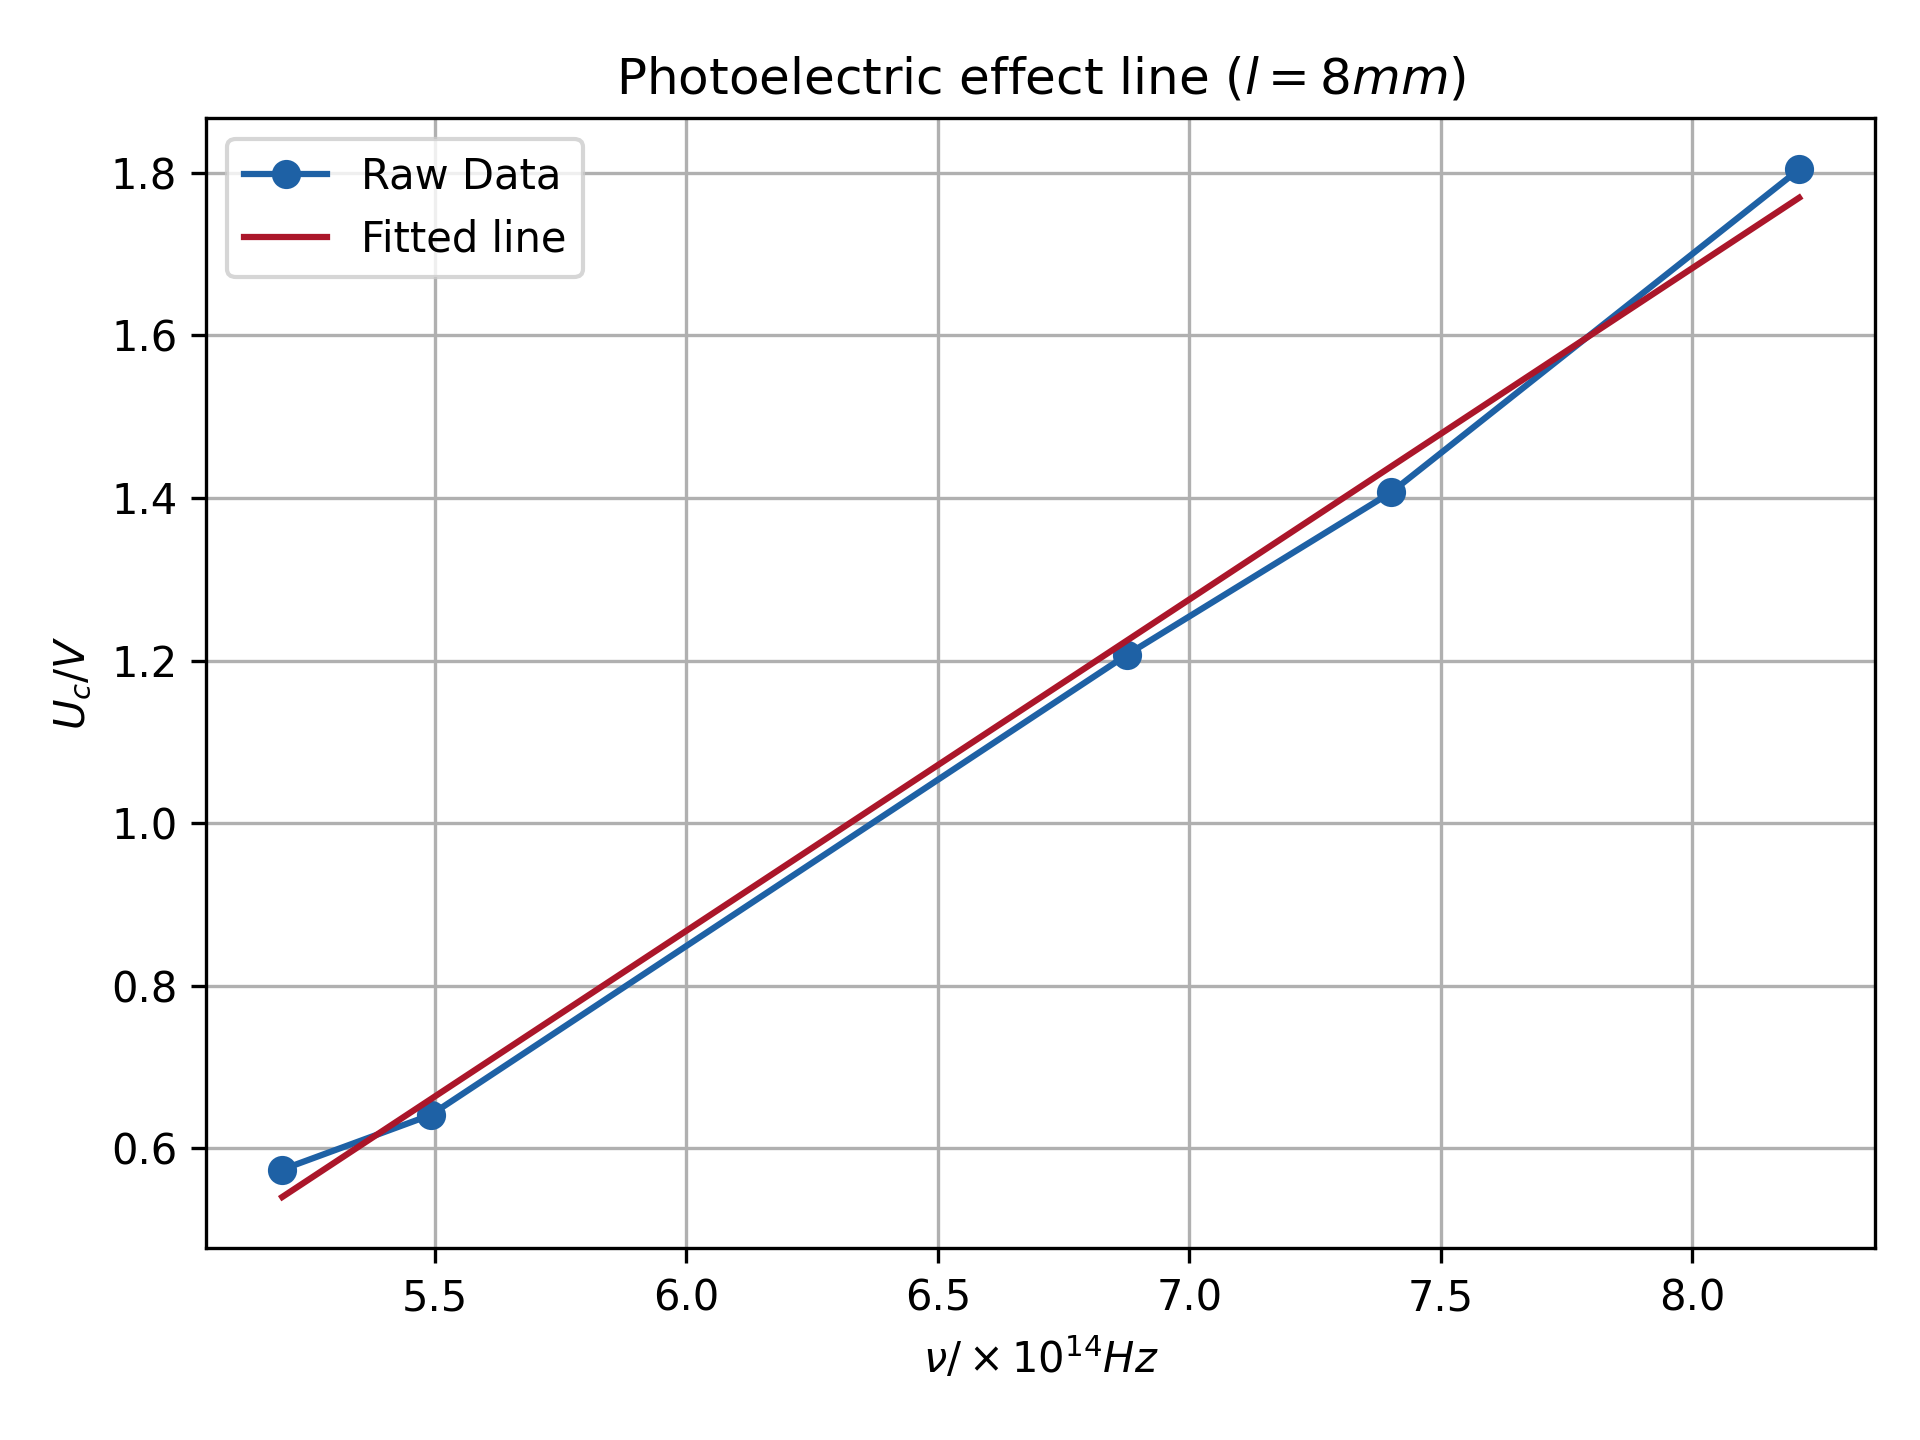
\includegraphics[width=\textwidth]{l_8.png}
        \caption{光阑孔直径 = 8 mm}
    \end{minipage}
\end{figure}

计算得到三个孔径下计算的普朗克常数$h$的值,以及与标准值的相对误差。

$$ \hat{h} = e \cdot k \qquad \varepsilon = \left|\frac{h-\hat{h}}{h}\right|\times 100\% $$
\begin{table}[!h]
    \centering
    \renewcommand{\arraystretch}{1.5}
    \begin{tabular}{|c|c|c|c|c|c|c|}
        \hline
        \multirow{2}{*}{光阑孔直径 $d \ (mm)$} & \multicolumn{3}{c|}{最小二乘} & \multicolumn{3}{c|}{作图法} \\
        \cline{2-7}
         & 2 & 4 & 8 & 2 & 4 & 8 \\
        \hline
        计算结果 $\hat{h} \ (\times 10^{-34} J \cdot s)$ & 6.484 & 6.537 & 6.517 & 6.666 & 6.565 & 6.523 \\
        \hline
        普朗克常数 $h \ (J \cdot s)$ & \multicolumn{6}{c|}{$6.626 \times 10^{-34}$} \\
        \hline
        相对误差 $\varepsilon$ & 2.13\% & 1.338\% & 1.642\% & 0.607\% & 0.914\% & 1.554\% \\
        \hline
    \end{tabular}
\end{table}

\section{实验结论以及现象分析}

%(分析实验误差的来源,以及比较以上每种数据处理方法的优缺点)

在测量普朗克常量的实验中,误差来源主要包括系统误差和随机误差。系统误差可能来自于仪器校准不准确、环境条件的变化(如温度、湿度)以及实验设备的非理想特性,例如光源的波长不稳定。随机误差则是由不可控因素引起的,如测量时的操作误差、环境噪声等。了解这些误差来源对于改进实验设计和提高测量精度至关重要。

在数据处理方法上,最小二乘法和作图法各有优缺点。最小二乘法通过最小化观测值与拟合直线之间的平方差,提供了一个精确的拟合结果,适用于处理大规模数据和复杂关系。它的优点在于能够量化拟合的优劣,并提供参数的标准误差,适合进行统计分析。然而,最小二乘法对于异常值敏感,可能会导致拟合结果的偏差。

相对而言,作图法直观易懂,能够快速展示数据的趋势,适合初步分析和小规模数据集。然而,作图法在量化拟合精度和处理复杂关系方面能力有限,且容易受到主观判断的影响,尤其在选择数据范围和线性化时。综合来看,选择合适的数据处理方法应根据具体实验要求和数据特性来决定,最小二乘法更适合精确测量,而作图法则更适合直观分析。

\section{讨论题}

\subsection{请解释什么是逸出功$A$,以及怎样可以从截止电压$U_0$与光频率$\nu$两者的线性关系中求出逸出功$W$。}

逸出功 $A$ 是指将电子从金属表面释放到真空所需克服的最小能量。这一概念与光电效应密切相关,光电效应指的是当光照射到金属表面时,能够使金属中的电子逸出。根据爱因斯坦的光电效应方程,实验中使用反向的电压来阻止电子的转移,故截止电压下电子的动能 $E_k$ 满足:

$$ eU_0 = E_k = h\nu - A $$

其中 \( e \) 是电子的电荷。将上述方程重排后可以得到:

$$ U_0 = \frac{h}{e}\nu - \frac{A}{e} $$

这个方程的形式类似直线方程,因此通过测量不同频率$\nu$下的截止电压$U_0$,可以绘制出 $U_0 \sim \nu$ 的线性关系图。根据拟合得到的截距可以计算出逸出功$A$:

$$ A = -e \times \text{截距} $$

通过这个方法,可以从截止电压 \( U_0 \) 与光频率 \( \nu \) 的线性关系中准确求出逸出功 \( A \)。

\subsection{请讨论一下,不同金属材料的逸出功$A$会否相同,并加以解释。}

不同金属材料的逸出功$A$通常不会相同,这主要是由于其电子结构的差异。每种金属的原子结构和电子排布各不相同,导致它们释放电子所需的能量不同。逸出功与金属的工作函数密切相关,而不同金属的工作函数受到其晶体结构、键合能及表面状态的影响。此外,金属表面的污染、氧化层或缺陷也会影响逸出功,不同金属在空气中的反应性和表面处理方式各异,可能导致表面状态的变化,进一步影响逸出功的测量。实验条件如温度和光源频率的变化也可能导致不同金属的逸出功表现不同。因此,选择不同金属材料时,需要考虑其逸出功的差异,这反映了材料的物理化学特性。

\subsection{请讨论一下,不同金属材料的$U_0 \sim \nu$线性关系会否相同,并加以解释。}

不同金属材料的 $U_0 \sim \nu$ 线性关系通常不会相同,这主要是因为不同金属的工作函数 $A$ 和电子结构的差异导致的。在前面的方程:

$$ U_0 = \frac{h}{e}\nu - \frac{A}{e} $$

\noindent 中,斜率 $\frac{h}{e}$ 是常量,与金属无关。然而,截距 $-\frac{A}{e}$ 直接取决于每种金属的逸出功 $A$。由于不同金属的逸出功值不同,导致不同金属的 $U_0$ 在相同频率 $\nu$ 下会有不同的值。这意味着,不同金属的 $U_0 \sim \nu$ 线性关系的截距会有所不同。

\subsection{请解释什么是暗电流、本底电流、和阳极反向电流,以及它们各自出现的原因,并讨论它们各自会怎样影响“零电流法”对截止电压$U_0$的测量结果。}

暗电流是指在无光照条件下,光电器件中流动的微弱电流,主要由热激发产生。它通常较小,但会影响测量精度。本底电流是由材料缺陷或环境噪声引起的电流,包含暗电流成分,进一步降低测量准确性。阳极反向电流是在反向电压下流动的电流,可能增加测量噪声。

在“零电流法”测量截止电压 $U_0$ 时,这些电流都会导致偏差。暗电流可能使 $U_0$ 测量值偏高,本底电流则可能导致假阳性,阳极反向电流则增加噪声。为提高测量准确性,需要对这些电流进行补偿或校正。

\end{document}